\chapter{Introduction}

\section{Motivation}
Revealing the structure of hierarchical organized data is a complex task where many approaches already exists (TODO cite). It is still an active research area as data scientists are facing ever greater challenges when analyzing large hierarchical datasets. One example is the Human Disease Network \cite{zhou_human_2014} which is a hierarchical network of disorders and disease genes with approximately 3000 nodes on two different hierarchy layers. Figure \ref{fig:Human_Disease_Network} shows us the representation of the data in a common two-dimensional layout, in this representation the classes of disorders are coded by color. 
Our own dataset with a similar structure can be seen in Figure \ref{fig:original2DdiseaseNet}, here the clusters of different diseases are grouped by boxes. Depiction of hierarchical network structure in 2D faces us with many challenges for example: 
\begin{itemize}
    \item \textbf{Limitation of visual features.} Figure \ref{fig:Human_Disease_Network} already uses the color to encode the group membership thus we can not use this feature to visualize additional attributes like mortality rate.
    \item \textbf{Lack of space.} A common problem in network visualization is the hairball effect, with only two dimensions the reduced space quickly leads to overlapping of nodes and links. In Figure \ref{fig:Human_Disease_Network} we can see this effect on the green nodes. The graph in Figure \ref{fig:original2DdiseaseNet} hides links between child nodes from different boxes to prevent overlapping which is also not optimal.
    \item \textbf{Restriction of spatial encoded data.} With only two available axes and therefore only two spatial encoded data attributes task like cluster detection and conformation are harder.
\end{itemize} 

\begin{figure}[h]
    \centering
    \begin{subfigure}[b]{0.4\columnwidth}
        \centering
        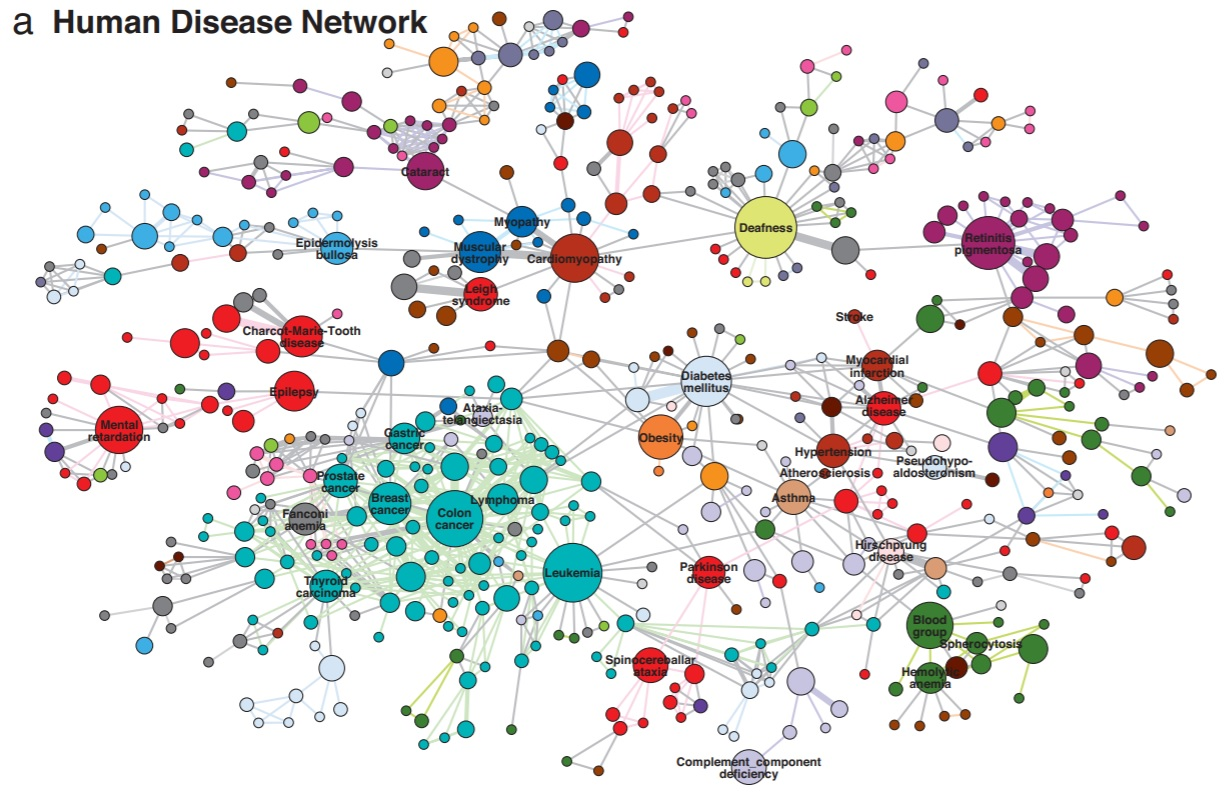
\includegraphics[width=\textwidth, trim={0 0 9cm 0},clip]{graphics/Human_Disease_Network.jpg}
        \subcaption{Human Disease Network \cite{zhou_human_2014}}
        \label{fig:Human_Disease_Network}
    \end{subfigure}
    \begin{subfigure}[b]{0.5\columnwidth}
      \centering
      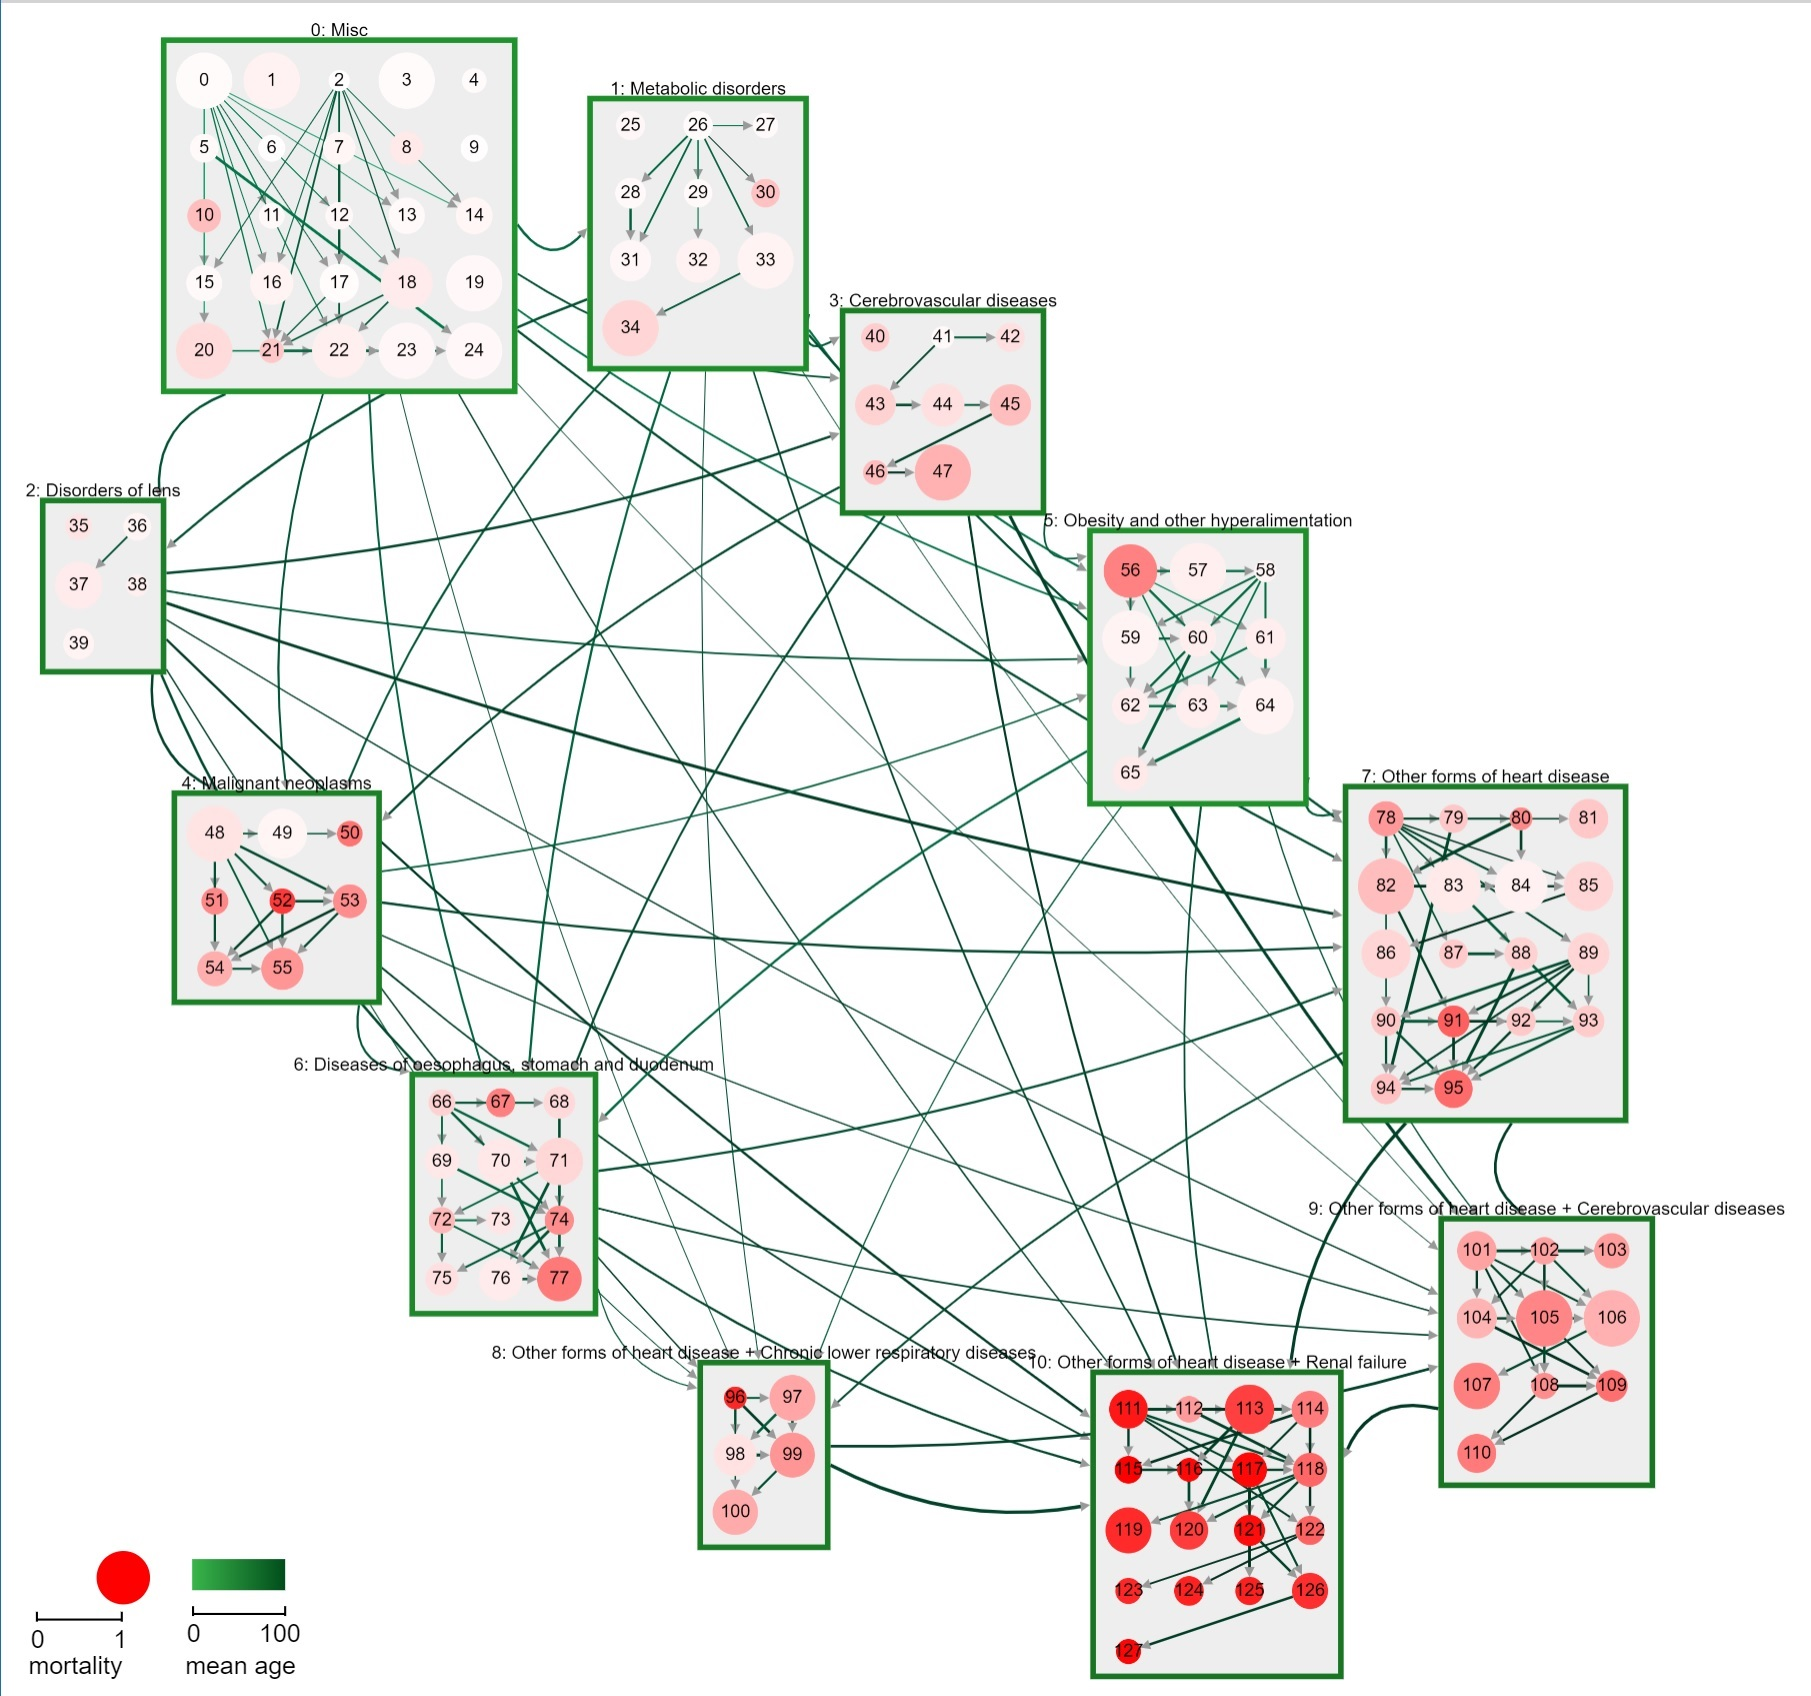
\includegraphics[width=\textwidth]{graphics/original2DdiseaseNet.jpg}
      \subcaption{Our own disease network dataset}
      \label{fig:original2DdiseaseNet}
    \end{subfigure}
    \caption[Optional caption for the figure list (often used to abbreviate long captions)]{Example visualizations of hierarchical network datasets in two dimensions. Both consists of two hierarchical layers.} % Remove the [...] argument if the original caption should be used in the figure list.
    \label{fig:intro} 
  \end{figure}

3D information visualization allows us to expand the user experience of traditional 2D graphs. As Brath describes in his paper \cite{brath_3d_2014} there are many advantages and opportunities when using three-dimensional visualizations.
The additional axes allow us to display an additional attribute by its position, this can be seen in the “3D space time cube” \cite{brath_3d_2014} here the temporal information is encoded on the Z axis another common usage is a 3D scatter plot. By using these additional spatial information the mental model gets improved. Furthermore, this results in a better understanding of the data by the user.
In the context of visual features we get a lot more of opportunities, one of the biggest is probably the ability to use surfaces and effects like shading. 
The perspective of the visualization can be reconsidered. Usually the user looks from the outside with a
bird's eye view at the visualization. In 3D however the viewer can be placed right inside our graph, this enables us to utilize new navigation and interaction possibilities. 

Still, all these opportunities also involve new challenges: navigation inside the visualization, occlusion of elements in an 3D perspective view, selection for displaying details and the lack of a reference point in three-dimensional space. Brath \cite{brath_3d_2014} already stated that immersive interfaces could help to overcome this issues.
 We believe that with the recent developments in virtual reality hardware and frameworks these challenges can now be solved even better. 
 We can see active research for this topic in various publications. Bowman et al. \cite{bowman_virtual_2007} research the impact of VR techniques like stereoscopic images, interaction with the virtual world and head movement can have on users. 
 Recently Kraus et al. \cite{kraus_impact_2020} did a study where they examined the effect of immersion for detecting clusters in a scatter plot. Their results show that VR based visualization systems have real world advantages in terms of time needed to get an overview of the data compared to traditional 2D- and 3D information visualization. In terms of navigation and interaction Yang et al. \cite{yang_embodied_2020} explored the possibility of zooming and rotation of an entire graph and Drogemuller \cite{drogemuller_examining_2020} compared different navigation concepts.
 
 \section{Methodology}
 \textbf{Starting idea: 2D Multilayer see figure, why not make use of all 3 axes in VR, instead of flat layers use 3D objects like cubes/spheres to bundle one layer} (Email 14.08.2020 https://arxiv.org/pdf/1902.06815.pdf)
 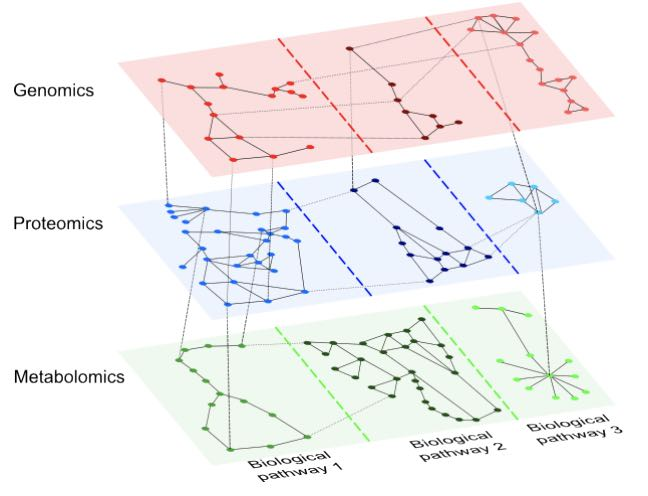
\includegraphics[width=0.5\textwidth]{chapters/graphics/2dmultilayerVis.jpg}
 
 Ideas:
 \begin{itemize}
     \item Example applications with hierarchical network data
     \item current 2D visualizations of hierarchical networks
     \item power of VR visualizations and board availability
 \end{itemize}

\section{Aim of the Work}
%From proposal: \\
%The	 goal	 is	 to	 visualize	 a	 hierarchical	 network	 with	 n	 Layers.	 Each	 Node	 in	 a	 graph	 can	
%represent	a	graph	itself.	There	are	multiple	examples	where	this	has	been	visualised	in	2D,	
%however	we	believe	that	with	an	additional	dimension	and	when	3D	graphs	are	analysed	in	
%VR	we	can	get	even	more	insight	and	a	better	overview	of	the	data.	

Ideas:
\begin{itemize}
    \item provide a prototype application
    \item benefits of webbased implementation 
    \item experiment with different concepts/approaches
    \item experiment with different interactions
    \item ...
\end{itemize}

\begin{quotation}
    However, there is considerable value in research that
    solves a well-motivated problem using a combination
    of preexisting solutions 
\end{quotation}
Sadana\\
Redefining a Contribution for Immersive Visualization Research\\

\section{Approach}



I want to give a short summary of chapter 4 proposed solution here. 

Ideas:
\begin{itemize}
    \item short description of planned final solution (web based, htc vive compatible, rendering multi hierarchical dataset, screenshot of solution)  
    \item short overview of used technologies and frameworks why? what it simplifies, ... 
    \item Customized Forces
    \item rendering, nodes inside parent, comparison to a default 2D Circle Packing plot https://observablehq.com/@d3/zoomable-circle-packing 
    \item available interactions
\end{itemize}